\section{Implementation}
\subsection{Algorithm}

The implemented algorithm receives as input a sequence of sonar positions
$\mathbf{P}_k$ and its respective sonar responses, that is a sequence of beams
$\mathbf{b}_j^{(k)}$ containing bearing and bins values. The procedure goes
as illustrated in Algorithm \ref{alg:mapping}.


\begin{algorithm}
\caption{Mapping}
\label{alg:mapping}
\begin{algorithmic}
\Procedure{Mapping}{$\mathbf{P}_k,\mathbf{b}_j^{(k)}$}

\State $I_k = \{\mathbf{b}_j^{(k)}|j\in \mu\mathbb{N}\}$
\Comment{Partitioning at every $\mu$ beam}

\State $\coord{w}_0 = \mathbf{0}$
\ForAll{$\mathbf{P}_k$}
\ForAll{$\mathbf{b}\in I_k$}
\State $\mathbf{b} = \mathrm{threshold}(\mathbf{b})$
\Comment{Classify empty/full, section \ref{s:ism}}
\State $e_i = \mathrm{empty\_samples}(\mathbf{b})$
\Comment{Sample first empty bins, section \ref{ss:isfm}}
\State $f_i^{(z)} = \mathrm{full\_samples}(\mathbf{b})$
\Comment{Sample from every $z$ full bin, section \ref{ss:isfm}}
\State $\text{feats}=\{\}$

\ForAll{$e_i$}
\State $\text{feats}=\text{feats}\cup\{\hat\varphi(e_i)\}$
\Comment{equation \ref{eq:nystrom}}
\EndFor

\ForAll{$f^{(z)}$}
\State
$\text{feats}=\text{feats}\cup\{\mathbb{E}_i[{
\hat\varphi(f_i^{(z)})}]\}$
\Comment{equation \ref{eq:embedding}}
\EndFor
\EndFor

\State $\coord{w} {-=}
\eta_k\nabla\text{NLL}_{\text{reg}}(\coord{w}_t;\text{feats})$ 
\Comment{equation \ref{eq:leariningrate} on a variant of
\ref{eq:minibatch}}
\EndFor
\State \textbf{return} $\coord{w}$
\EndProcedure
\end{algorithmic}
\end{algorithm}

In the description of the algorithm
$\nabla\text{NLL}_{\text{reg}}(\coord{w}_t;\text{feats})$ has a slightly
different meaning:

\begin{equation*}
\nabla\text{NLL}_{\text{reg}}(\coord{w}_t;\text{feats}) =
\sum_{\hat{\mathbf{\varphi}}\in \text{feats}}
-y_t\hat{\mathbf{\varphi}}(1+\exp(y_i~ \coord{w}\cdot\hat{\mathbf{\varphi}})^{-1} +\lambda\nabla\mathcal{S}(\coord{w})
\end{equation*}


\subsection{Results}

Although the algorithm generates a 3D representation of an environment, results
displayed here are plane cuts of this reconstruction only for better
appreciation. The environment considered here is the 4x5 semi-inifinity box of
section \ref{eq:boxlikenv}. There were used $3000$ inducing points (dimension of
the feature map approximation - section \ref{sss:hilbertcontinuousmap}) and $21$
measurements from $7$ different positions in $3$ ortogonal orientations each
from the sonar simulation. Different fractions of the number of beams were
explored on figures \ref{fig:ten_map}, \ref{fig:thir_map} and
\ref{fig:full_map}. Colors represent the value of the occupancy
$p(x;\coord{w})$.

\begin{figure}[ht]
    \centering
    \subfloat[Plane
    $x=-1$]{{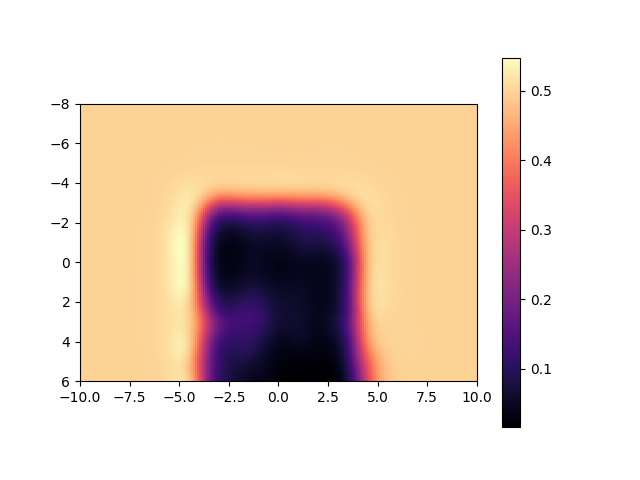
\includegraphics[width=75mm,trim={0 14mm 0
    10mm},clip]{Chap4/fig/ten_x_-1}}}%
    \hfill \subfloat[Plane
    $z=-2$]{{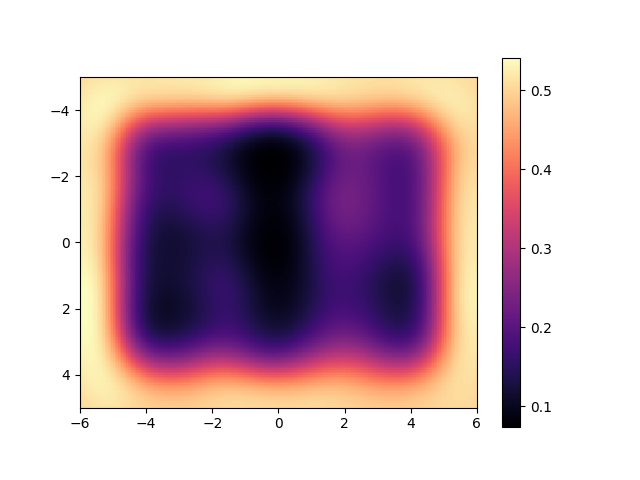
\includegraphics[width=75mm,trim={0 14mm 0
    10mm},clip]{Chap4/fig/ten_z_-2}}}%
    \\%
    \subfloat[Plane
    $x=0$]{{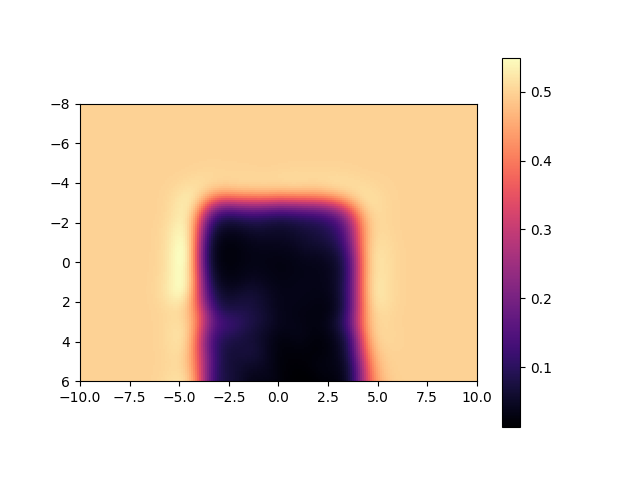
\includegraphics[width=75mm,trim={0 14mm 0
    10mm},clip]{Chap4/fig/ten_x_0}}}%
    \hfill \subfloat[Plane
    $z=-1$]{{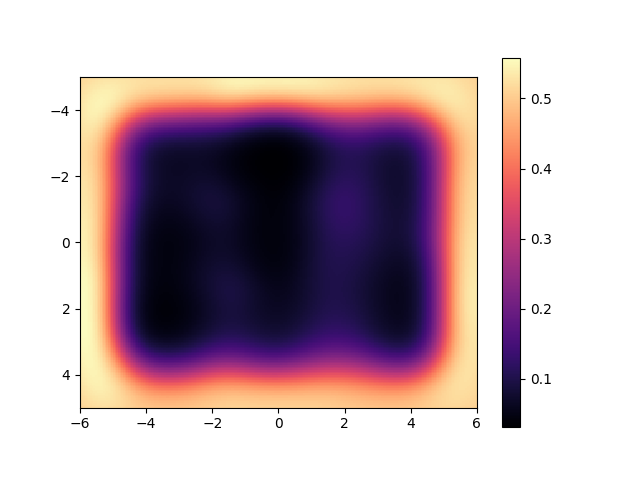
\includegraphics[width=75mm,trim={0 14mm 0
    10mm},clip]{Chap4/fig/ten_z_-1}}}%
    \\%
    \subfloat[Plane
    $x=1$]{{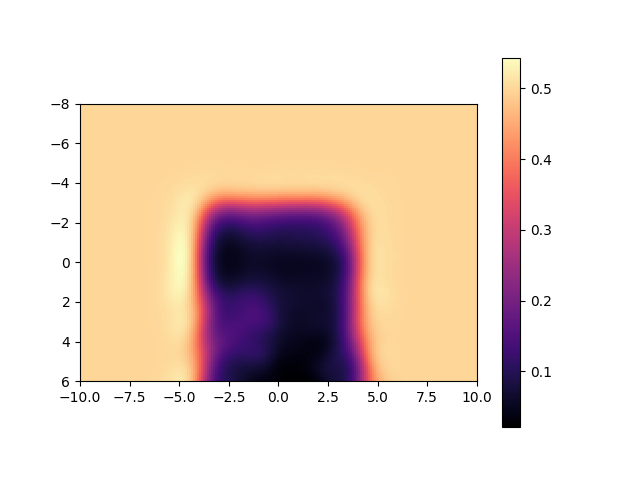
\includegraphics[width=75mm,trim={0 14mm 0
    10mm},clip]{Chap4/fig/ten_x_1}}}%
    \hfill \subfloat[Plane
    $z=0$]{{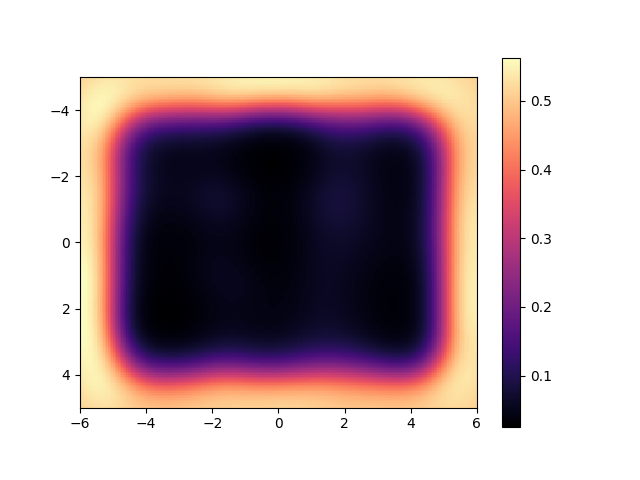
\includegraphics[width=75mm,trim={0 14mm 0
    10mm},clip]{Chap4/fig/ten_z_0}}}%
    \caption{Mapping with $10\%$ of available beams.}%
    \label{fig:ten_map}%
\end{figure}

\begin{figure}[ht]
    \centering
    \subfloat[Plane
    $x=-1$]{{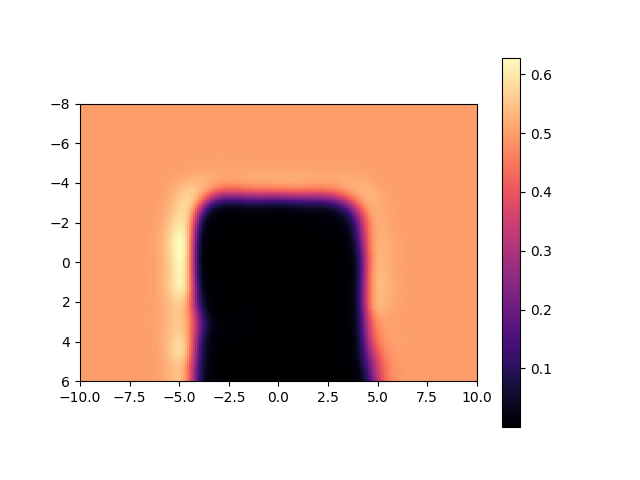
\includegraphics[width=75mm,trim={0 14mm 0
    10mm},clip]{Chap4/fig/thir_x_-1}}}%
    \hfill \subfloat[Plane
    $z=-2$]{{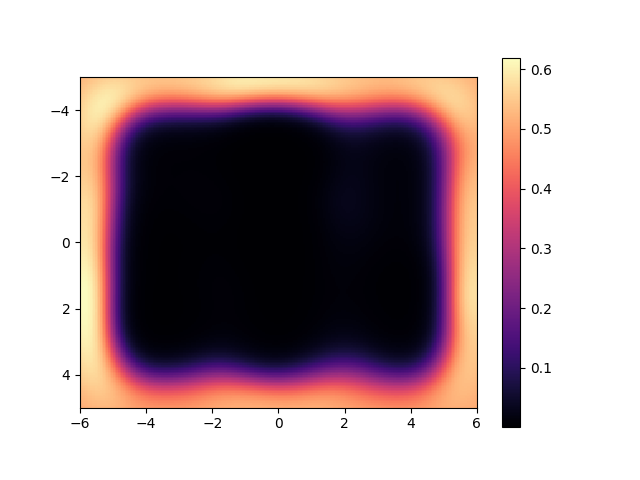
\includegraphics[width=75mm,trim={0 14mm 0
    10mm},clip]{Chap4/fig/thir_z_-2}}}%
    \\%
    \subfloat[Plane
    $x=0$]{{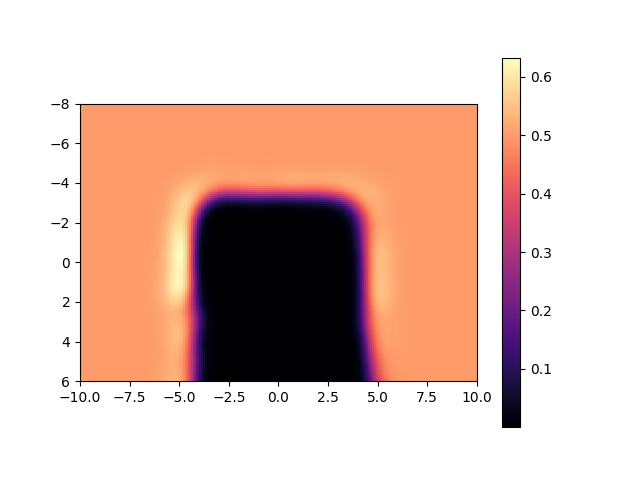
\includegraphics[width=75mm,trim={0 14mm 0
    10mm},clip]{Chap4/fig/thir_x_0}}}%
    \hfill \subfloat[Plane
    $z=-1$]{{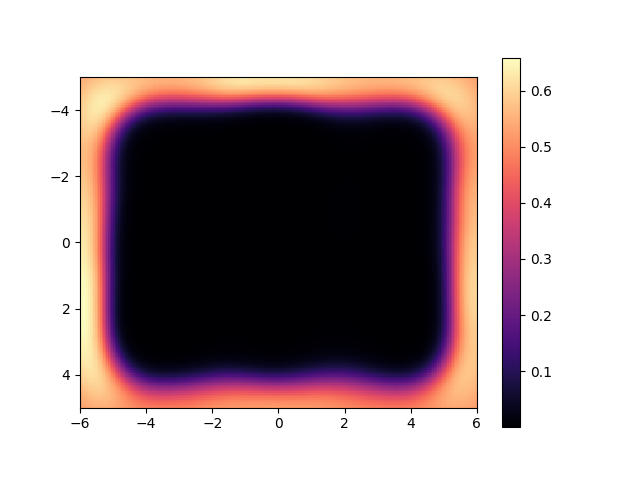
\includegraphics[width=75mm,trim={0 14mm 0
    10mm},clip]{Chap4/fig/thir_z_-1}}}%
    \\%
    \subfloat[Plane
    $x=1$]{{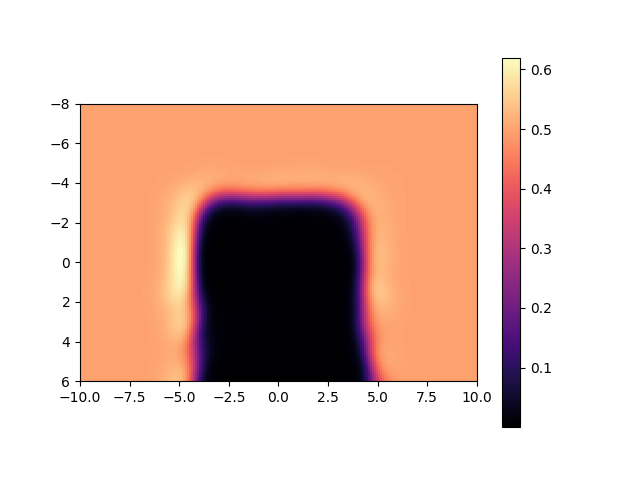
\includegraphics[width=75mm,trim={0 14mm 0
    10mm},clip]{Chap4/fig/thir_x_1}}}%
    \hfill \subfloat[Plane
    $z=0$]{{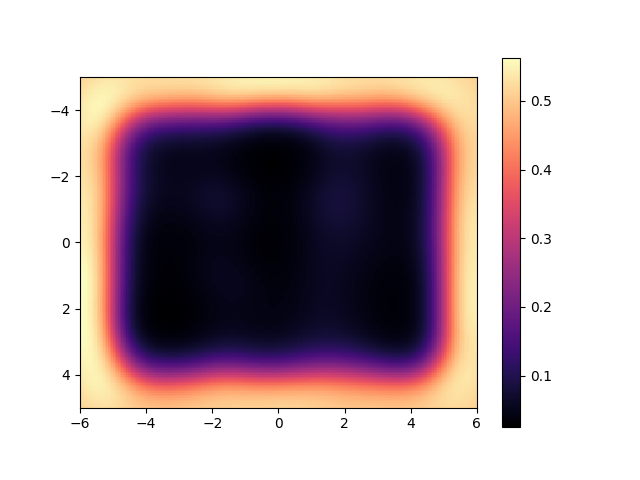
\includegraphics[width=75mm,trim={0 14mm 0
    10mm},clip]{Chap4/fig/ten_z_0}}}%
    \caption{Mapping with $30\%$ of available beams.}%
    \label{fig:thir_map}%
\end{figure}

\begin{figure}[ht]
    \centering
    \subfloat[Plane
    $x=-1$]{{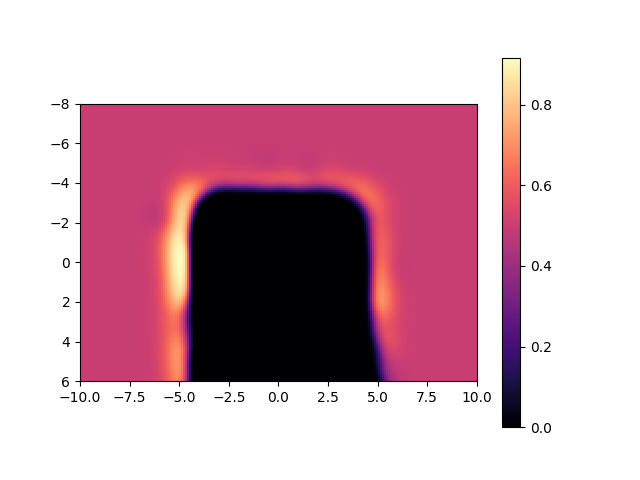
\includegraphics[width=75mm,trim={0 14mm 0
    10mm},clip]{Chap4/fig/full_x_-1}}}%
    \hfill \subfloat[Plane
    $z=-2$]{{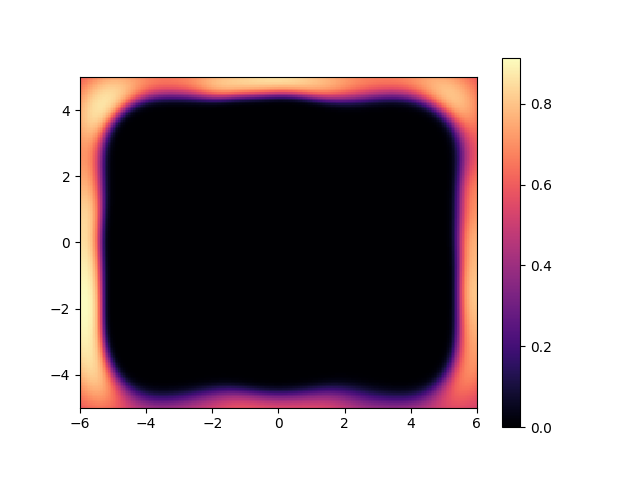
\includegraphics[width=75mm,trim={0 14mm 0
    10mm},clip]{Chap4/fig/full_z_-2}}}%
    \\%
    \subfloat[Plane
    $x=0$]{{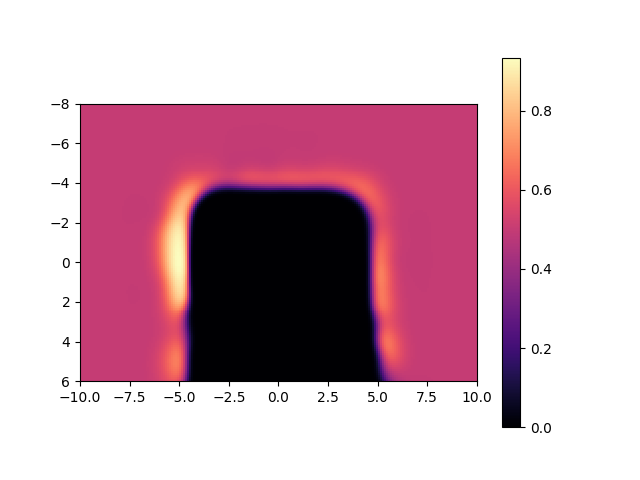
\includegraphics[width=75mm,trim={0 14mm 0
    10mm},clip]{Chap4/fig/full_x_0}}}%
    \hfill \subfloat[Plane
    $z=-1$]{{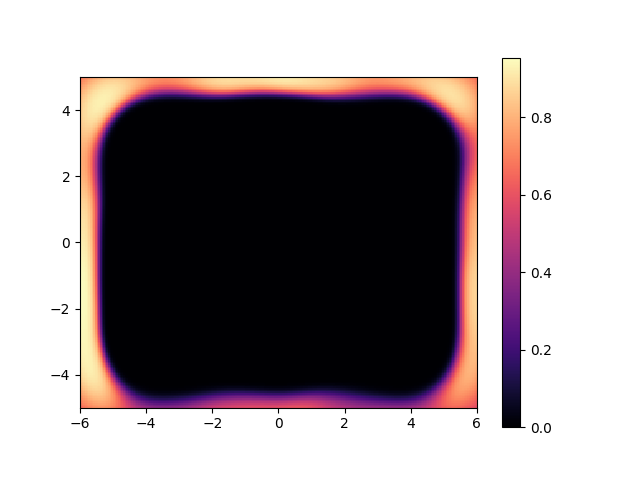
\includegraphics[width=75mm,trim={0 14mm 0
    10mm},clip]{Chap4/fig/full_z_-1}}}%
    \\%
    \subfloat[Plane
    $x=1$]{{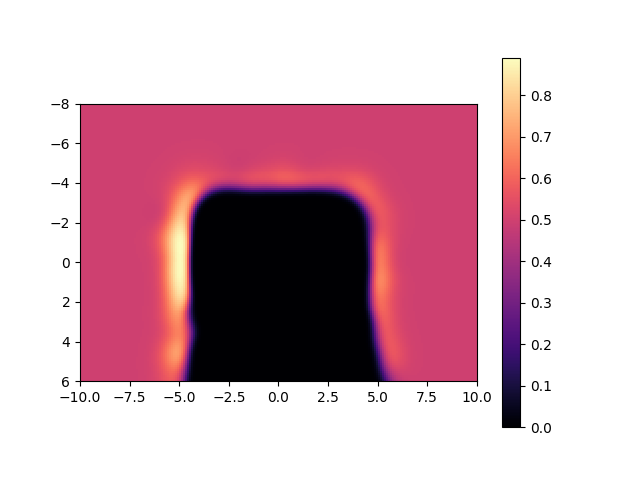
\includegraphics[width=75mm,trim={0 14mm 0
    10mm},clip]{Chap4/fig/full_x_1}}}%
    \hfill \subfloat[Plane
    $z=0$]{{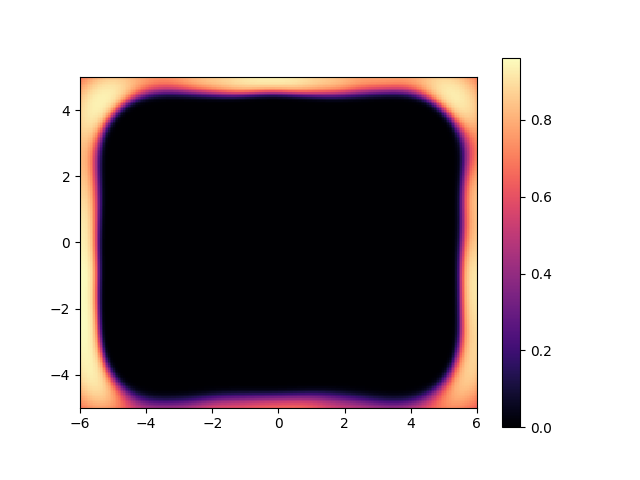
\includegraphics[width=75mm,trim={0 14mm 0
    10mm},clip]{Chap4/fig/full_z_0}}}%
    \caption{Mapping with $100\%$ of available beams.}%
    \label{fig:full_map}%
\end{figure}
